\documentclass[conference]{IEEEtran}
\usepackage{amsmath,amssymb,graphicx,booktabs,url}
\title{Spatial and Temporal RIS Control with a Coupled Electromagnetic Reference}
\author{\IEEEauthorblockN{Atom-wise RIS Research}\IEEEauthorblockA{Development pilot --- 24 October 2026}}
\begin{document}\maketitle
\begin{abstract}
We compare atom-wise learned mutation and temporal network prediction using a numerically checked, 3D coupled electromagnetic model. A 64-element wire surface, four transmitting antennas and two moving receivers are solved together using the NEC-2 thin-wire method of moments. Exact multiport reduction and low-rank updates are shared by analytical and learned controllers. Twelve trajectories are split before label generation, with three optimizer seeds and complete CPU budgets from 1 to 100 ms. The primary budget is selected on validation cases. This is a free-space wire-reference development study, not a calibrated OpenSourceRIS PCB model, a measured experiment, or a final paper test.
\end{abstract}
\section{Question and scope}
Spatial intelligence chooses useful joint edits among interacting elements. Temporal intelligence forecasts a changing environment from causal history. They address different problems and must not be conflated. Existing multiport theory, full-wave validation and efficient physical channel computation provide the foundations~\cite{nerini,abrardo,prod}; coupling itself is not a new contribution. Experimental coupling calibration already exists~\cite{zheng}, and analytical discrete optimization remains a strong competitor~\cite{hammami}.

The previous independent-cell Munich experiment favored cached pair search. Here we replace that approximate surface with an explicitly specified wire benchmark. Both geometry and hardware model change, so comparing absolute rates with Munich would not isolate coupling.

\section{Electromagnetic reference}
All 70 wires are modeled in a shared free-space scene at 5.53 GHz. Every wire is 24 mm long, with radius 50 $\mu$m; the RIS pitches are 28 mm horizontally and 30 mm vertically. Wires are perfectly conducting, vertically polarized and have center ports. The binary loads are $1-j10.799~\Omega$ and $1+j129.201~\Omega$. There is no substrate, ground plane, real switch, conductor loss, city geometry, or human-body blockage. Receiver motion changes the electromagnetic network.

Unit-voltage excitations yield the complete admittance matrix and its inverse $Z$. All external references are real 50 $\Omega$. Let $L$ contain RIS loads and external terminations. The off-diagonal transmit-to-receive power-wave channel is
\begin{equation}
 H=-100[(Z+L)^{-1}]_{RT}.
\end{equation}
A Schur complement reduces repeated solves to the RIS block; rank-one and rank-two Woodbury updates evaluate bit edits exactly. The source precoder is all-OFF-reference regularized zero forcing, fixed during optimization. Its total incident power is 0.1 W; this is not a claim of 0.1 W radiated power. The objective is the weakest user's $\log_2(1+\mathrm{SINR})$, with interference, 1 MHz bandwidth, 290 K and 7 dB noise figure.

\begin{figure*}[t]\centering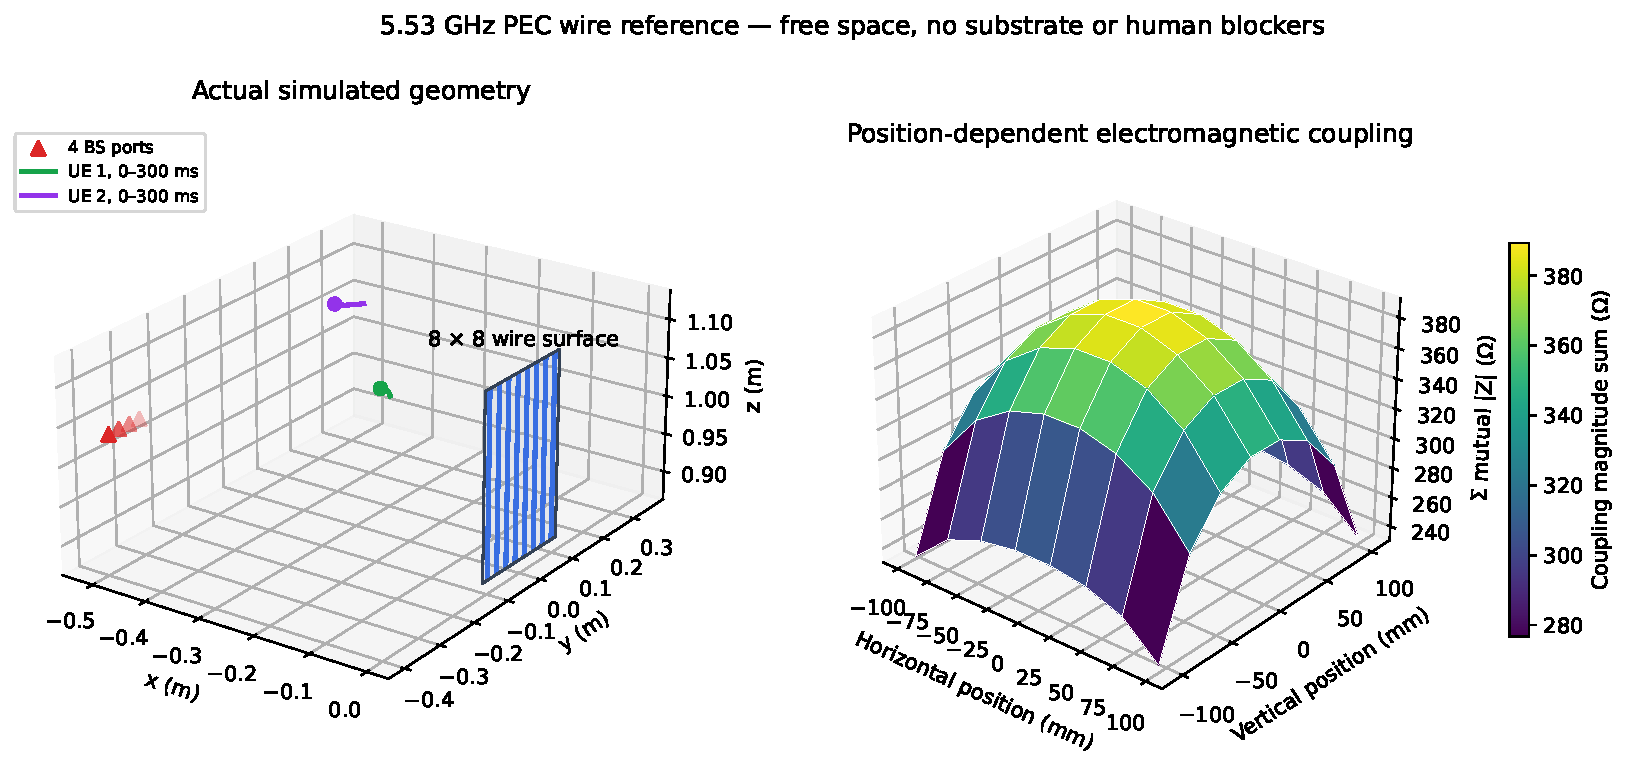
\includegraphics[width=\textwidth]{figures/geometry_3d.pdf}\caption{Actual simulated geometry and the position-dependent sum of mutual impedance magnitudes. The height map is a coupling diagnostic, not a received-power or measured field map.}\label{fig:geometry}\end{figure*}

The production mesh has 81 segments per wire (5,670 unknowns); the refinement has 161 (11,270). Over 103 reference patterns, maximum complex-channel change is 0.740\%, and maximum rate change is 0.01503 bit/s/Hz. Direct loaded NEC solves agree with network-reduced currents to $7.41\times10^{-14}$ relative norm. Passivity is checked per generated frame; reciprocity and loaded-response checks are recorded. Numerical convergence does not establish fabricated-device accuracy.

\section{Data and matched comparisons}
Twelve complete trajectories have 16 frames at 20 ms spacing. Six trajectories train, three validate and three form a development pilot. They share one surface and scene; this is not environmental generalization. All splits precede labels. Enumeration of 2,016 pairs per parent yields 2,304 training and 1,152 validation examples, including conditional pair targets with harmful first flips. Of 1,152 inspected parents, 524 single-bit local optima admit beneficial pairs.

Spatial tests use current network observations. Greedy, pair, random search, memory GA, analytically guided GA, shared MLP and atom attention share the physical evaluator. The MLP has 14,113 parameters. Attention has two layers, width 32, four heads and 17,665 parameters. Both add learned corrections to analytical flip scores, with matched GA population 12, memory 8, crossover probability 0.25 and a 50/50 mixture of one and two distinct flips. Attention uses per-atom physics features without an explicit graph-edge bias. The ``no physics'' ablation removes additional complex/coupling features while retaining analytical gains; it is not a physics-free controller.

Coupling-blind pair search removes inter-RIS off-diagonal impedance only in its internal evaluator. Its reference precoder is shared with other controllers, and all returned actions are scored on the same fully coupled truth. This isolates the optimizer's model mismatch, not every possible use of coupling information.

Temporal tests receive four perfect past impedance observations and predict the next 20 ms frame. Persistence and linear extrapolation compete with a shared 1,090-parameter GRU. Forecast matrices are projected to passive reciprocal matrices. All causal methods and the current-CSI oracle use the same stale-reference precoder. MLP and attention are tested under both persistence and GRU predictions. Prior spatio-temporal channel-prediction work motivates the comparison~\cite{liu}; our target is downstream rate after computational overhead, not prediction loss alone.

Complete network observations are idealized. Their acquisition cost, practical identifiability and microcontroller implementation are not demonstrated. The oracle has extra current information and is not a global optimization upper bound.

\section{CPU results}
All methods run sequentially on one CPU core with one BLAS/Torch thread. Budgets are 1, 5, 10, 50 and 100 ms. Forecasting, projection, precoding, network setup, features, memory, inference and candidate evaluation are timed; model loading, channel acquisition, EM generation and subsequent environmental action scoring are excluded. Candidates completed after the deadline cannot improve the returned action. Validation selected 10 ms. Seeds are 7, 19 and 43.
\begin{table}[t]\centering\caption{Spatial control: current CSI}\small\begin{tabular}{lrrr}\toprule Controller & Rate & p95 (ms) & Misses\\\midrule
pair & 17.1022 & 8.99 & 0/144 \\
analytical\_ga & 16.9080 & 9.32 & 0/144 \\
greedy & 16.7752 & 9.11 & 0/144 \\
attention\_no\_physics\_ga & 16.7687 & 8.99 & 0/144 \\
attention\_ga & 16.7650 & 8.92 & 0/144 \\
attention\_no\_memory\_ga & 16.7650 & 8.96 & 0/144 \\
memory\_ga & 16.7650 & 9.27 & 0/144 \\
mlp\_ga & 16.7650 & 8.56 & 0/144 \\
random & 16.7650 & 9.15 & 0/144 \\
blind\_pair & 6.0254 & 9.00 & 0/144 \\
\bottomrule\end{tabular}\end{table}
\begin{table}[t]\centering\caption{Temporal control: 20 ms stale CSI}\small\begin{tabular}{lrrr}\toprule Controller & Rate & p95 (ms) & Misses\\\midrule
oracle\_pair & 15.6395 & 9.04 & 0/108 \\
linear\_pair & 5.1270 & 9.00 & 0/108 \\
gru\_attention\_ga & 5.0682 & 8.91 & 0/108 \\
gru\_mlp\_ga & 5.0229 & 8.60 & 0/108 \\
persistence\_pair & 4.7815 & 8.98 & 0/108 \\
persistence\_attention\_ga & 4.7641 & 8.95 & 0/108 \\
persistence\_mlp\_ga & 4.7641 & 8.58 & 0/108 \\
gru\_pair & 4.6664 & 9.05 & 0/108 \\
\bottomrule\end{tabular}\end{table}

\begin{figure*}[t]\centering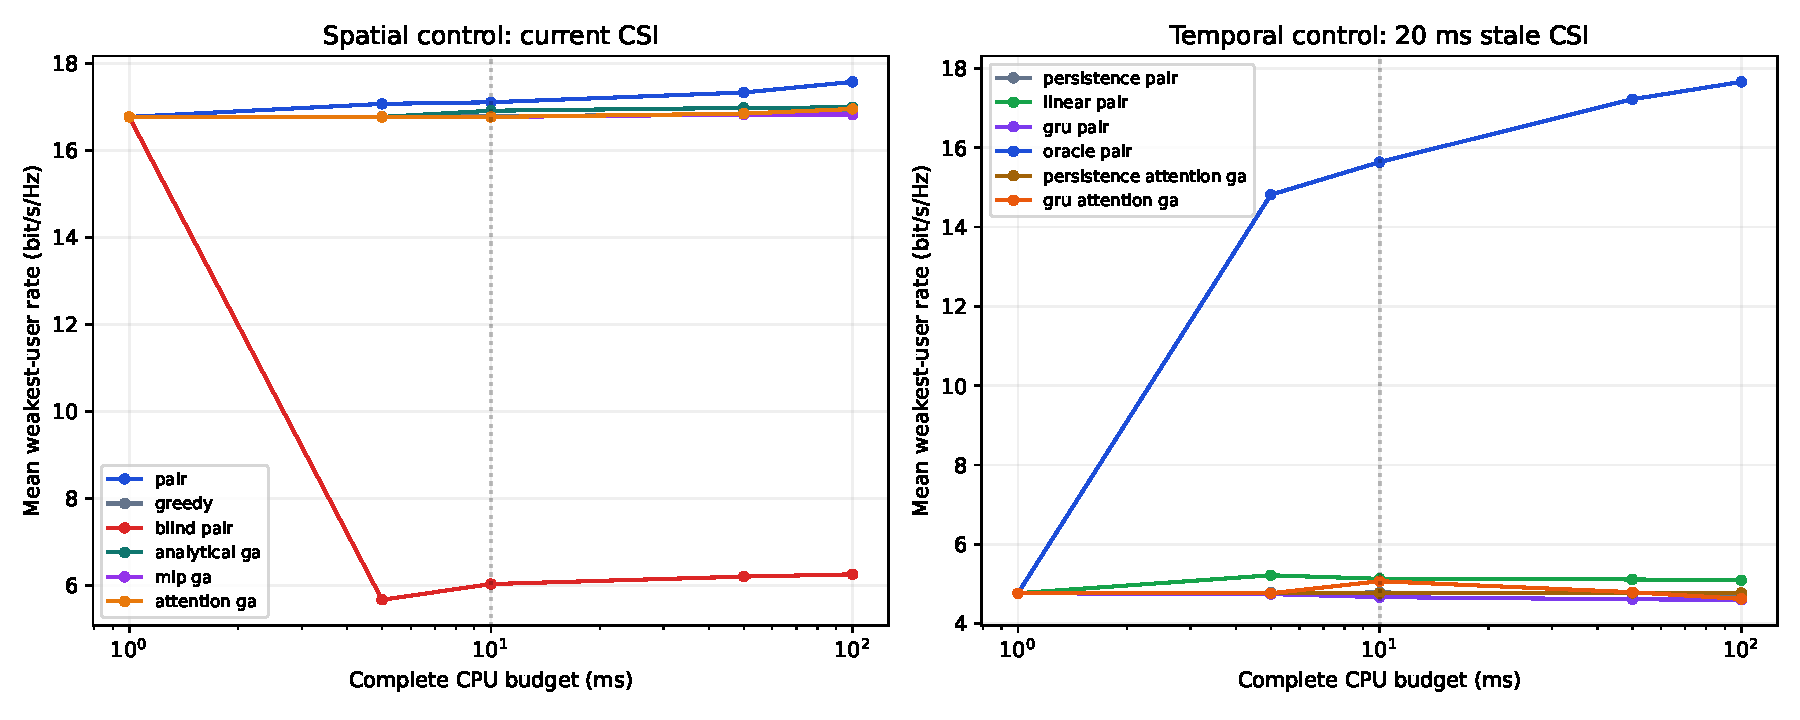
\includegraphics[width=\textwidth]{figures/rate_runtime.pdf}\caption{Development-pilot rate versus complete controller budget. Curves include all recorded trials; deadline misses are separately reported.}\end{figure*}

Paired differences average frames and seeds within each trajectory first:
\begin{itemize}
\item attention\_ga versus pair: -0.3372 bit/s/Hz (descriptive interval [-0.7898, -0.0291]).
\item pair versus blind\_pair: +11.0768 bit/s/Hz (descriptive interval [+10.3713, +11.6191]).
\item gru\_pair versus persistence\_pair: -0.1151 bit/s/Hz (descriptive interval [-1.3990, +0.6172]).
\item linear\_pair versus persistence\_pair: +0.3454 bit/s/Hz (descriptive interval [+0.0134, +0.6928]).
\item gru\_pair versus linear\_pair: -0.4606 bit/s/Hz (descriptive interval [-1.7291, +0.4229]).
\item gru\_attention\_ga versus persistence\_attention\_ga: +0.3041 bit/s/Hz (descriptive interval [-0.3876, +0.8804]).
\end{itemize}
Only three pilot trajectories are independent. The bootstrap intervals are descriptive, not sufficient evidence of general superiority.

\section{Mesh sensitivity of returned actions}
At one predeclared pilot frame per mode, all methods' returned actions and seeds are rescored with the 161-segment network and the original precoder frozen. Across 54 actions, maximum relative channel discrepancy is 0.523\% and maximum rate discrepancy is 0.64381 bit/s/Hz. No action is reoptimized during this audit. Small algorithm gaps must be judged against these numerical differences; one-frame checks do not certify every trajectory.

\section{Research decision and remaining evidence}
At 10 ms, spatial pair search achieves 17.1022 bit/s/Hz versus 16.7650 for attention. Under stale CSI, linear prediction plus pair search achieves 5.1270, versus 4.6664 for GRU plus pair search. GRU plus attention achieves 5.0682. The present attention policy does not establish an advantage over analytical search. This does not rule out better spatial architectures or better supervision.

The numerical model makes an honest coupling experiment possible, but it does not establish that attention is necessary. The results should select the simplest controller that delivers comparable held-out utility after overhead. Any spatial gain must survive matched analytical search; any temporal gain must survive persistence and linear forecasting. The saved report contains the complete tables, paired differences and per-method deadline counts.

Before a broader novelty claim, expand to independent geometries and trajectories, noisy or partial channel observations, multiple mobility and delay regimes, and an untouched final evaluation. For a faithful OpenSourceRIS study, obtain a PCB/substrate/switch full-wave model or mixed-pattern multiport calibration. Two uniform-surface ON/OFF curves do not identify the neighbor-coupling matrix.

\section*{Reproducibility}
Code, reports, figures and metadata are available at \url{https://github.com/ElFariss/atom-wise-ris}. Large generated arrays and checkpoints are retained in the local/lab workspace and excluded from Git. Source and data hashes, seeds, model histories and raw controller records are preserved. All 28 literature-matrix entries retain their reading statuses.

\begin{thebibliography}{6}
\bibitem{nerini} M. Nerini et al., ``A universal framework for multiport network analysis of reconfigurable intelligent surfaces,'' \emph{IEEE TWC}, 2024, doi: 10.1109/TWC.2024.3416825.
\bibitem{abrardo} A. Abrardo, A. Toccafondi, and M. Di Renzo, ``Design of reconfigurable intelligent surfaces by using S-parameter multiport network theory---Optimization and full-wave validation,'' \emph{IEEE TWC}, 2024, doi: 10.1109/TWC.2024.3450722.
\bibitem{prod} H. Prod'homme and P. del Hougne, ``Efficient computation of physics-compliant channel realizations for (rich-scattering) RIS-parametrized radio environments,'' \emph{IEEE Communications Letters}, 2023, doi: 10.1109/LCOMM.2023.3330527.
\bibitem{zheng} P. Zheng et al., ``Mutual coupling in RIS-aided communication: Model training and experimental validation,'' \emph{IEEE TWC}, 2024, doi: 10.1109/TWC.2024.3451548.
\bibitem{hammami} C. Hammami, L. Le Magoarou, and P. del Hougne, ``Statistical multiport-network modeling and efficient discrete optimization of RIS,'' \emph{IEEE WCL}, 2026, doi: 10.1109/LWC.2026.3652464.
\bibitem{liu} G. Liu et al., ``Spatio-temporal neural network for channel prediction in massive MIMO-OFDM systems,'' \emph{IEEE Transactions on Communications}, 2022, doi: 10.1109/TCOMM.2022.3215198.
\end{thebibliography}
\end{document}
